\begin{frame}{Πειραματικά αποτελέσματα: WILLOWGARAGE (sim; 4/6)}

  \begin{figure}
    \definecolor{a}{RGB}{235, 172, 35}
\definecolor{b}{RGB}{184, 0, 88}
\definecolor{c}{RGB}{0, 140, 249}
\definecolor{d}{RGB}{0, 110, 0}
\definecolor{e}{RGB}{0, 187, 173}
\definecolor{f}{RGB}{209, 99, 230}
\definecolor{g}{RGB}{178, 69, 2}
\definecolor{h}{RGB}{255, 146, 135}
\definecolor{i}{RGB}{89, 84, 214}
\definecolor{j}{RGB}{135, 133, 0}

% GNUPLOT: LaTeX picture with Postscript
\begingroup
  \makeatletter
  \providecommand\color[2][]{%
    \GenericError{(gnuplot) \space\space\space\@spaces}{%
      Package color not loaded in conjunction with
      terminal option `colourtext'%
    }{See the gnuplot documentation for explanation.%
    }{Either use 'blacktext' in gnuplot or load the package
      color.sty in LaTeX.}%
    \renewcommand\color[2][]{}%
  }%
  \providecommand\includegraphics[2][]{%
    \GenericError{(gnuplot) \space\space\space\@spaces}{%
      Package graphicx or graphics not loaded%
    }{See the gnuplot documentation for explanation.%
    }{The gnuplot epslatex terminal needs graphicx.sty or graphics.sty.}%
    \renewcommand\includegraphics[2][]{}%
  }%
  \providecommand\rotatebox[2]{#2}%
  \@ifundefined{ifGPcolor}{%
    \newif\ifGPcolor
    \GPcolorfalse
  }{}%
  \@ifundefined{ifGPblacktext}{%
    \newif\ifGPblacktext
    \GPblacktexttrue
  }{}%
  % define a \g@addto@macro without @ in the name:
  \let\gplgaddtomacro\g@addto@macro
  % define empty templates for all commands taking text:
  \gdef\gplfronttext{}%
  \gdef\gplfronttext{}%
  \makeatother
  \ifGPblacktext
    % no textcolor at all
    \def\colorrgb#1{}%
    \def\colorgray#1{}%
  \else
    % gray or color?
    \ifGPcolor
      \def\colorrgb#1{\color[rgb]{#1}}%
      \def\colorgray#1{\color[gray]{#1}}%
      \expandafter\def\csname LTw\endcsname{\color{white}}%
      \expandafter\def\csname LTb\endcsname{\color{black}}%
      \expandafter\def\csname LTa\endcsname{\color{black}}%
      \expandafter\def\csname LT0\endcsname{\color[rgb]{1,0,0}}%
      \expandafter\def\csname LT1\endcsname{\color[rgb]{0,1,0}}%
      \expandafter\def\csname LT2\endcsname{\color[rgb]{0,0,1}}%
      \expandafter\def\csname LT3\endcsname{\color[rgb]{1,0,1}}%
      \expandafter\def\csname LT4\endcsname{\color[rgb]{0,1,1}}%
      \expandafter\def\csname LT5\endcsname{\color[rgb]{1,1,0}}%
      \expandafter\def\csname LT6\endcsname{\color[rgb]{0,0,0}}%
      \expandafter\def\csname LT7\endcsname{\color[rgb]{1,0.3,0}}%
      \expandafter\def\csname LT8\endcsname{\color[rgb]{0.5,0.5,0.5}}%
    \else
      % gray
      \def\colorrgb#1{\color{black}}%
      \def\colorgray#1{\color[gray]{#1}}%
      \expandafter\def\csname LTw\endcsname{\color{white}}%
      \expandafter\def\csname LTb\endcsname{\color{black}}%
      \expandafter\def\csname LTa\endcsname{\color{black}}%
      \expandafter\def\csname LT0\endcsname{\color{black}}%
      \expandafter\def\csname LT1\endcsname{\color{black}}%
      \expandafter\def\csname LT2\endcsname{\color{black}}%
      \expandafter\def\csname LT3\endcsname{\color{black}}%
      \expandafter\def\csname LT4\endcsname{\color{black}}%
      \expandafter\def\csname LT5\endcsname{\color{black}}%
      \expandafter\def\csname LT6\endcsname{\color{black}}%
      \expandafter\def\csname LT7\endcsname{\color{black}}%
      \expandafter\def\csname LT8\endcsname{\color{black}}%
    \fi
  \fi
    \setlength{\unitlength}{0.0500bp}%
    \ifx\gptboxheight\undefined%
      \newlength{\gptboxheight}%
      \newlength{\gptboxwidth}%
      \newsavebox{\gptboxtext}%
    \fi%
    \setlength{\fboxrule}{0.5pt}%
    \setlength{\fboxsep}{1pt}%
\begin{picture}(9500.00,4000.00)%
    \gplgaddtomacro\gplfronttext{%
      \colorrgb{0.15,0.15,0.15}%
      \put(822,1666){\makebox(0,0)[r]{\strut{}\footnotesize 35}}%
      \colorrgb{0.15,0.15,0.15}%
      \put(822,1876){\makebox(0,0)[r]{\strut{}\footnotesize 40}}%
      \colorrgb{0.15,0.15,0.15}%
      \put(822,2086){\makebox(0,0)[r]{\strut{}\footnotesize 45}}%
      \colorrgb{0.15,0.15,0.15}%
      \put(822,2296){\makebox(0,0)[r]{\strut{}\footnotesize 50}}%
      \colorrgb{0.15,0.15,0.15}%
      \put(822,2506){\makebox(0,0)[r]{\strut{}\footnotesize 55}}%
      \colorrgb{0.15,0.15,0.15}%
      \put(822,2717){\makebox(0,0)[r]{\strut{}\footnotesize 60}}%
      \colorrgb{0.15,0.15,0.15}%
      \put(822,2927){\makebox(0,0)[r]{\strut{}\footnotesize 65}}%
      \colorrgb{0.15,0.15,0.15}%
      \put(822,3137){\makebox(0,0)[r]{\strut{}\footnotesize 70}}%
      \colorrgb{0.15,0.15,0.15}%
      \put(822,3347){\makebox(0,0)[r]{\strut{}\footnotesize 75}}%
      \colorrgb{0.15,0.15,0.15}%
      \put(822,3557){\makebox(0,0)[r]{\strut{}\footnotesize 80}}%
      \colorrgb{0.15,0.15,0.15}%
      \put(954,1446){\makebox(0,0){\strut{}\footnotesize 45}}%
      \colorrgb{0.15,0.15,0.15}%
      %\put(1164,1446){\makebox(0,0){\strut{}\footnotesize 50}}%
      \colorrgb{0.15,0.15,0.15}%
      \put(1374,1446){\makebox(0,0){\strut{}\footnotesize 55}}%
      \colorrgb{0.15,0.15,0.15}%
      %\put(1584,1446){\makebox(0,0){\strut{}\footnotesize 60}}%
      \colorrgb{0.15,0.15,0.15}%
      \put(1794,1446){\makebox(0,0){\strut{}\footnotesize 65}}%
      \colorrgb{0.15,0.15,0.15}%
      %\put(2005,1446){\makebox(0,0){\strut{}\footnotesize 70}}%
      \colorrgb{0.15,0.15,0.15}%
      \put(2215,1446){\makebox(0,0){\strut{}\footnotesize 75}}%
      \colorrgb{0.15,0.15,0.15}%
      %\put(2425,1446){\makebox(0,0){\strut{}\footnotesize 80}}%
      \colorrgb{0.15,0.15,0.15}%
      \put(2635,1446){\makebox(0,0){\strut{}\footnotesize 85}}%
      \colorrgb{0.15,0.15,0.15}%
      %\put(2845,1446){\makebox(0,0){\strut{}\footnotesize 90}}%
    }%
    \gplgaddtomacro\gplfronttext{%
      \colorrgb{0.15,0.15,0.15}%
      \put(316,2632){\rotatebox{90}{\makebox(0,0){\strut{}$y$ [m]}}}%
      \colorrgb{0.15,0.15,0.15}%
      \put(1899,1116){\makebox(0,0){\strut{}$x$ [m]}}%
      \put(1699,600){\makebox(0,0){\strut{} \footnotesize $|\mathcal{H}_G| = 500$ υποθέσεις (1 υπ./4.0 m$^2$)}}%
      \put(1699,300){\makebox(0,0){\strut{} \footnotesize $100 \times \{\bm{p}_i\} = 1000$ απόπειρες εκτίμησης}}%
    }%
    \gplgaddtomacro\gplfronttext{%
      \colorrgb{0.15,0.15,0.15}%
      \put(3668,2933){\makebox(0,0)[r]{\strut{}\scriptsize $0\%$}}%
      \colorrgb{0.15,0.15,0.15}%
      \put(3668,3100){\makebox(0,0)[r]{\strut{}\scriptsize $25\%$}}%
      \colorrgb{0.15,0.15,0.15}%
      \put(3668,3266){\makebox(0,0)[r]{\strut{}\scriptsize $50\%$}}%
      \colorrgb{0.15,0.15,0.15}%
      \put(3668,3433){\makebox(0,0)[r]{\strut{}\scriptsize $75\%$}}%
      \colorrgb{0.15,0.15,0.15}%
      \put(3668,3599){\makebox(0,0)[r]{\strut{}\scriptsize $100\%$}}%
      \colorrgb{0.15,0.15,0.15}%
      \put(3895,2813){\makebox(0,0){\strut{}\scriptsize \textcolor{a}{$\bm{p}_a^G$}}}%
      \colorrgb{0.15,0.15,0.15}%
      \put(4085,2813){\makebox(0,0){\strut{}\scriptsize \textcolor{b}{$\bm{p}_b^G$}}}%
      \colorrgb{0.15,0.15,0.15}%
      \put(4275,2813){\makebox(0,0){\strut{}\scriptsize \textcolor{c}{$\bm{p}_c^G$}}}%
      \colorrgb{0.15,0.15,0.15}%
      \put(4465,2813){\makebox(0,0){\strut{}\scriptsize \textcolor{d}{$\bm{p}_d^G$}}}%
      \colorrgb{0.15,0.15,0.15}%
      \put(4655,2813){\makebox(0,0){\strut{}\scriptsize \textcolor{e}{$\bm{p}_e^G$}}}%
      \colorrgb{0.15,0.15,0.15}%
      \put(4844,2813){\makebox(0,0){\strut{}\scriptsize \textcolor{f}{$\bm{p}_f^G$}}}%
      \colorrgb{0.15,0.15,0.15}%
      \put(5034,2813){\makebox(0,0){\strut{}\scriptsize \textcolor{g}{$\bm{p}_g^G$}}}%
      \colorrgb{0.15,0.15,0.15}%
      \put(5224,2813){\makebox(0,0){\strut{}\scriptsize \textcolor{h}{$\bm{p}_h^G$}}}%
      \colorrgb{0.15,0.15,0.15}%
      \put(5414,2813){\makebox(0,0){\strut{}\scriptsize \textcolor{i}{$\bm{p}_i^G$}}}%
      \colorrgb{0.15,0.15,0.15}%
      \put(5604,2813){\makebox(0,0){\strut{}\scriptsize \textcolor{j}{$\bm{p}_j^G$}}}%
    }%
    \gplgaddtomacro\gplfronttext{%
      \colorrgb{0.00,0.00,0.00}%
      \put(6000,3819){\makebox(0,0){\strut{}\footnotesize Ποσοστά αποτυχιών}}%
      \put(4700,4219){\makebox(0,0){\strut{}\footnotesize Μέσω \texttt{PLICP}}}%
      \put(7500,4219){\makebox(0,0){\strut{}\footnotesize Μέσω \texttt{FMI-SPOMF}}}%

    }%
    \gplgaddtomacro\gplfronttext{%
      \colorrgb{0.15,0.15,0.15}%
      \put(6518,2933){\makebox(0,0)[r]{\strut{}\scriptsize $0\%$}}%
      \colorrgb{0.15,0.15,0.15}%
      \put(6518,3100){\makebox(0,0)[r]{\strut{}\scriptsize $25\%$}}%
      \colorrgb{0.15,0.15,0.15}%
      \put(6518,3266){\makebox(0,0)[r]{\strut{}\scriptsize $50\%$}}%
      \colorrgb{0.15,0.15,0.15}%
      \put(6518,3433){\makebox(0,0)[r]{\strut{}\scriptsize $75\%$}}%
      \colorrgb{0.15,0.15,0.15}%
      \put(6518,3599){\makebox(0,0)[r]{\strut{}\scriptsize $100\%$}}%
      \colorrgb{0.15,0.15,0.15}%
      \put(6745,2813){\makebox(0,0){\strut{}\scriptsize \textcolor{a}{$\bm{p}_a^G$}}}%
      \colorrgb{0.15,0.15,0.15}%
      \put(6935,2813){\makebox(0,0){\strut{}\scriptsize \textcolor{b}{$\bm{p}_b^G$}}}%
      \colorrgb{0.15,0.15,0.15}%
      \put(7125,2813){\makebox(0,0){\strut{}\scriptsize \textcolor{c}{$\bm{p}_c^G$}}}%
      \colorrgb{0.15,0.15,0.15}%
      \put(7315,2813){\makebox(0,0){\strut{}\scriptsize \textcolor{d}{$\bm{p}_d^G$}}}%
      \colorrgb{0.15,0.15,0.15}%
      \put(7505,2813){\makebox(0,0){\strut{}\scriptsize \textcolor{e}{$\bm{p}_e^G$}}}%
      \colorrgb{0.15,0.15,0.15}%
      \put(7694,2813){\makebox(0,0){\strut{}\scriptsize \textcolor{f}{$\bm{p}_f^G$}}}%
      \colorrgb{0.15,0.15,0.15}%
      \put(7884,2813){\makebox(0,0){\strut{}\scriptsize \textcolor{g}{$\bm{p}_g^G$}}}%
      \colorrgb{0.15,0.15,0.15}%
      \put(8074,2813){\makebox(0,0){\strut{}\scriptsize \textcolor{h}{$\bm{p}_h^G$}}}%
      \colorrgb{0.15,0.15,0.15}%
      \put(8264,2813){\makebox(0,0){\strut{}\scriptsize \textcolor{i}{$\bm{p}_i^G$}}}%
      \colorrgb{0.15,0.15,0.15}%
      \put(8454,2813){\makebox(0,0){\strut{}\scriptsize \textcolor{j}{$\bm{p}_j^G$}}}%
    }%
    \gplgaddtomacro\gplfronttext{%
    }%
    \gplgaddtomacro\gplfronttext{%
      \colorrgb{0.15,0.15,0.15}%
      \put(3668,1666){\makebox(0,0)[r]{\strut{}\scriptsize $0.0$}}%
      \colorrgb{0.15,0.15,0.15}%
      \put(3668,1809){\makebox(0,0)[r]{\strut{}\scriptsize $0.30$}}%
      \colorrgb{0.15,0.15,0.15}%
      \put(3668,1951){\makebox(0,0)[r]{\strut{}\scriptsize $0.60$}}%
      \colorrgb{0.15,0.15,0.15}%
      \put(3668,2094){\makebox(0,0)[r]{\strut{}\scriptsize $0.90$}}%
      \colorrgb{0.15,0.15,0.15}%
      \put(3668,2237){\makebox(0,0)[r]{\strut{}\scriptsize $1.2$}}%
      \colorrgb{0.15,0.15,0.15}%
      \put(3717,1546){\makebox(0,0){\strut{}\scriptsize $\sigma_R$:}}%
      \put(4117,1546){\makebox(0,0){\strut{}\scriptsize $0.01$}}%
      \colorrgb{0.15,0.15,0.15}%
      \put(4750,1546){\makebox(0,0){\strut{}\scriptsize $0.02$}}%
      \colorrgb{0.15,0.15,0.15}%
      \put(5383,1546){\makebox(0,0){\strut{}\scriptsize $0.05$}}%
    }%
    \gplgaddtomacro\gplfronttext{%
      \colorrgb{0.00,0.00,0.00}%
      \put(6000,2552){\makebox(0,0){\strut{}\footnotesize Μέσο σφάλμα στάσης [$(\text{m}^2 + \text{rad}^2)^{1/2}$]}}%
    }%
    \gplgaddtomacro\gplfronttext{%
      \colorrgb{0.15,0.15,0.15}%
      \put(6518,1666){\makebox(0,0)[r]{\strut{}\scriptsize $0.0$}}%
      \colorrgb{0.15,0.15,0.15}%
      \put(6518,1856){\makebox(0,0)[r]{\strut{}\scriptsize $0.10$}}%
      \colorrgb{0.15,0.15,0.15}%
      \put(6518,2047){\makebox(0,0)[r]{\strut{}\scriptsize $0.20$}}%
      \colorrgb{0.15,0.15,0.15}%
      \put(6518,2237){\makebox(0,0)[r]{\strut{}\scriptsize $0.30$}}%
      \colorrgb{0.15,0.15,0.15}%
      \put(6567,1546){\makebox(0,0){\strut{}\scriptsize $\sigma_R$:}}%
      \put(6967,1546){\makebox(0,0){\strut{}\scriptsize $0.01$}}%
      \colorrgb{0.15,0.15,0.15}%
      \put(7600,1546){\makebox(0,0){\strut{}\scriptsize $0.02$}}%
      \colorrgb{0.15,0.15,0.15}%
      \put(8233,1546){\makebox(0,0){\strut{}\scriptsize $0.05$}}%
    }%
    \gplgaddtomacro\gplfronttext{%
    }%
    \gplgaddtomacro\gplfronttext{%
      \colorrgb{0.15,0.15,0.15}%
      %\put(3668,400){\makebox(0,0)[r]{\strut{}\scriptsize $50$}}%
      \colorrgb{0.15,0.15,0.15}%
      \put(3668,495){\makebox(0,0)[r]{\strut{}\scriptsize $100$}}%
      \colorrgb{0.15,0.15,0.15}%
      %\put(3668,590){\makebox(0,0)[r]{\strut{}\scriptsize $150$}}%
      \colorrgb{0.15,0.15,0.15}%
      \put(3668,685){\makebox(0,0)[r]{\strut{}\scriptsize $200$}}%
      \colorrgb{0.15,0.15,0.15}%
      %\put(3668,781){\makebox(0,0)[r]{\strut{}\scriptsize $250$}}%
      \colorrgb{0.15,0.15,0.15}%
      \put(3668,876){\makebox(0,0)[r]{\strut{}\scriptsize $300$}}%
      \colorrgb{0.15,0.15,0.15}%
      %\put(3668,971){\makebox(0,0)[r]{\strut{}\scriptsize $350$}}%
      \colorrgb{0.15,0.15,0.15}%
      \put(3668,1066){\makebox(0,0)[r]{\strut{}\scriptsize $400$}}%
      \colorrgb{0.15,0.15,0.15}%
      \put(3717,280){\makebox(0,0){\strut{}\scriptsize $\sigma_R$:}}%
      \put(4117,280){\makebox(0,0){\strut{}\scriptsize $0.01$}}%
      \colorrgb{0.15,0.15,0.15}%
      \put(4750,280){\makebox(0,0){\strut{}\scriptsize $0.02$}}%
      \colorrgb{0.15,0.15,0.15}%
      \put(5383,280){\makebox(0,0){\strut{}\scriptsize $0.05$}}%
    }%
    \gplgaddtomacro\gplfronttext{%
      \colorrgb{0.00,0.00,0.00}%
      \put(6000,1286){\makebox(0,0){\strut{}\footnotesize Μέσος χρόνος εκτέλεσης ανά υπόθεση [ms]}}%
    }%
    \gplgaddtomacro\gplfronttext{%
      \colorrgb{0.15,0.15,0.15}%
      %\put(6518,400){\makebox(0,0)[r]{\strut{}\scriptsize $50$}}%
      \colorrgb{0.15,0.15,0.15}%
      \put(6518,495){\makebox(0,0)[r]{\strut{}\scriptsize $100$}}%
      \colorrgb{0.15,0.15,0.15}%
      %\put(6518,590){\makebox(0,0)[r]{\strut{}\scriptsize $150$}}%
      \colorrgb{0.15,0.15,0.15}%
      \put(6518,685){\makebox(0,0)[r]{\strut{}\scriptsize $200$}}%
      \colorrgb{0.15,0.15,0.15}%
      %\put(6518,781){\makebox(0,0)[r]{\strut{}\scriptsize $250$}}%
      \colorrgb{0.15,0.15,0.15}%
      \put(6518,876){\makebox(0,0)[r]{\strut{}\scriptsize $300$}}%
      \colorrgb{0.15,0.15,0.15}%
      %\put(6518,971){\makebox(0,0)[r]{\strut{}\scriptsize $350$}}%
      \colorrgb{0.15,0.15,0.15}%
      \put(6518,1066){\makebox(0,0)[r]{\strut{}\scriptsize $400$}}%
      \colorrgb{0.15,0.15,0.15}%
      \put(6567,280){\makebox(0,0){\strut{}\scriptsize $\sigma_R$:}}%
      \put(6967,280){\makebox(0,0){\strut{}\scriptsize $0.01$}}%
      \colorrgb{0.15,0.15,0.15}%
      \put(7600,280){\makebox(0,0){\strut{}\scriptsize $0.02$}}%
      \colorrgb{0.15,0.15,0.15}%
      \put(8233,280){\makebox(0,0){\strut{}\scriptsize $0.05$}}%
    }%
    \gplgaddtomacro\gplfronttext{%
    }%
    \put(0,0){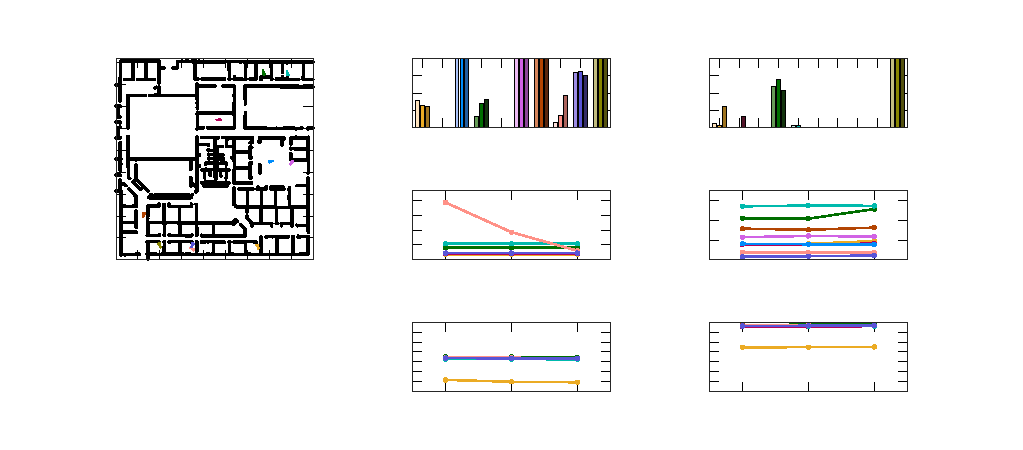
\includegraphics{./figures/slides/ch5/experiments//results_willowgarage}}%
    \gplfronttext
  \end{picture}%
\endgroup

  \end{figure}


\note{\footnotesize
Στο περιβάλλον WILLOGARAGE φαίνεται πως ο plicp απαιτεί οι στάσεις από τις
  οποίες συλλαμβάνονται οι δύο μετρήσεις να έχουν μικρή απόσταση μεταξύ τους
  ώστε να είναι ικανός να τις ευθυγραμμίσει, και πως το ίδιόν του κριτήριο
  επιλογής τελικής στάσης δεν είναι ικανό να ξεδιαλύνει ασάφειες, όπως δηλαδή
  στο περιβάλλον HOME.}
\end{frame}
